\documentclass[10pt,twocolumn,letterpaper]{article}
\usepackage{graphicx}
\graphicspath{ {./} }

\begin{document}

%%%%%%%%% TITLE
\title{Predicting a Film's Rating Utilizing Machine Learning}

\author{Joel Martinez\\
Texas State University\\
\and
Jose Garcia\\
Texas State University\\
\and
Kameron Bush\\
Texas State University\\\\
}
\maketitle
%\thispagestyle{empty}

%%%%%%%%% ABSTRACT
\begin{abstract}
	We present a program that will utilize existing data on films that have been released in order to predict
	the rating of a film that has yet to be released. This prediction will be given to the film industries that created the film in order to give them a chance to improve the film if needed. The factors being used are IMDB rating, budget, USA gross, USA opening weekend gross, tomatometer, metascore, and worldwide gross. We used using linear regression, k-nearest neighbors, and logistic regression as our model for the project. K-nearest neighbors and logistic regression will utilize k-fold cross validation and will be used as a contender against our linear model. Our methodology to solve this problem included intense research and rigorous testing.
\end{abstract}

%%%%%%%%% BODY TEXT
\section{Problem Description}
	When a film industry decides to create a film, the creators have to factor in many attributes that are important to how the public will interpret and perceive the film. Some of these factors are the company’s film budget, the film critic ratings, and how much the film makes on its first weekend.\\
	This public interpretation is very important to the film company because how the public perceives the film ultimately determines how many people go and see the film. The amount of people who go see the movie ultimately determines if the film company makes a profit off of the movie, i.e. if it is a ‘hit’ or a ‘flop’.\\
	The fate of the film cannot be determined until after the film is released to the public making it too late to make any changes if it fails. Our program is aimed to fix this problem by analyzing factors of previous films in order to predict the audience rating the new film will receive. This audience rating will give the film company a general idea of how well their film will do before they release the movie. Based on the audience rating presented, the film company will be able to fix their film before release so they can maybe save the film from flopping.\\ The film industry is a staple in many cultures. It affects almost anyone you can think of. This, along with the fact that we are big fans of films and what it takes to create a work of art worth seeing, is what pushed us to pursue this problem.

%-------------------------------------------------------------------------
\section{Survey}
	To see how much of an impact this project would have with the general population, we asked 50 students their opinion.\\\\
	Q: Do you believe this project will have an impact on which movies you will watch based on the rating generated?\\\\
	37 students said it would have an impact.\\
	9 students said it would not impact them.\\
	4 students said they did not know.

%-------------------------------------------------------------------------
\section{Plan}
	March 8th - Understand the Problem in-depth\\
	- Our group has got a now gotten a better understanding of how we can attack this problem. Our attributes will be able to help us use our model to estimate the probability of success (IMBD Rating, Budget, USA Gross, USA Opening Weekend Gross, Tomatometer, Metascore, Worldwide Gross).\\\\
	March 14th - Develop a data base for the code\\
	- We first created a database where we stored our x attributes and our y audience rating (1.0-10.0) in excel.\\\\
	March 25th - Complete a base algorithm for Project\\
	- Our model first takes the data from the database (excel), then splits our data to a X and Y dataset. Our model will consist of a train/test split of the X and Y dataset. We used Linear Regression to find a relation between the X attributes and the rating, we then proceeded to use the K-Fold method to optimize our model.\\\\
	March 29th - Complete Intermediate Project Report\\
	- Done and done.\\\\
	April 10th - Research ways to make algorithm more accurate\\
	- This step took us some time. We found that doubling the size of our dataset was the most influential change that increased the accuracy of our models.\\\\
	April 20th - Edit algorithm to be more effective and more precise\\
	- We implemented cross validation in our k-nearest neighbors and logistic regression models in order to increase the precision of our predictor. In the end we saw an increase of about 20\% using cross validation but our linear regression model continued to be the more accurate model of the three.\\\\
	April 29th - Complete Final Project Presentation\\
	- Done.\\\\
	May 4th - Complete Final Project Report\\
	- This report is proof of completion.

%-------------------------------------------------------------------------
\section{Data}
	The data set contains seven attributes (or features, denoted by X1. . . X8) and
	one response (or outcomes, denoted by y1). The aim is to use these seven
	features to predict the outcome.\\
	We specifically choose these seven features because the information is easy to find
	and open to the public. Some other attributes that we considered for the data was
	harder to come across on the internet and left many holes in our data. This would have
	required us to have to clean our data beforehand. With the attributes we are using
	there is no need to clean the data because we handpicked each movie individually to
	contain all or most of the attributes.\\
	Data was obtained from the Rotten Tomatoes website which provided us with the
	Tomatometer (Rotten Tomatoe's score of the movie), and the audience score (the value
	that we intend to predict.) We also utilized the IMDb website to obtain the gross USA
	(the amount of money that was made in the USA), the gross opening weekend USA (the amount
	of money that was made in the first week that the movie was released to the public),
	worldwide gross (the total amount of money made around the globe), budget (the amount of
	money the studio spent to create the movie), metascore (the IMDb user's score of the
	film), and IMDb rating (the score that IMDb critics gave the film.)\\ All this would come together to predict what an average person watching the film would rate it. Because this score is given by a person and not so calculating machine these scores have an entropic nature. Some may give a low score while others may give a high score. To combat this problem, we have simple stuck to the audience score from Rotten Tomatoes that takes the average of all user's scores. 
	\\\\Specifically:\\
	\\*X1 Gross USA\\
	\\*X2 Gross Opening Weekend USA\\
	\\*X3 Worldwide Gross\\
	\\*X4 Budget\\
	\\*X5 Metascore\\
	\\*X6 IMDb rating\\
	\\*X7 Tomatometer\\
	\\*y1 Audience Score\\\\
	
	Below is a screenshot of the first few lines in the dataset that we are utilizing for our
	model. As you can see, most attributes are filled in and few are null. We intend to expand
	the size of the dataset as we continue to work on the project. Much of the data is gathered
	by hand and requires a large amount of time to find. Fortunately, the doubling of our dataset was enough to increase our accuracy dramatically so we felt that there was not much benefit in adding much more data to our set.
	
	\begin{center}
		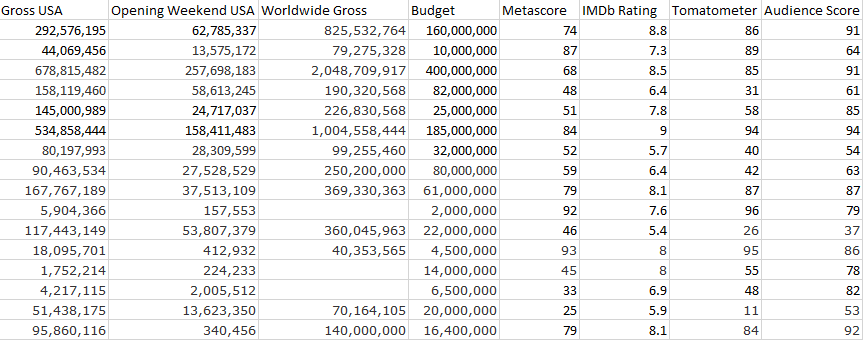
\includegraphics[width=8.5cm,height=6.95cm]{moviedatashot}
	\end{center}

%-------------------------------------------------------------------------
\section{Results}
	\begin{center}
		\includegraphics[scale=0.75]{linregshot}
		\includegraphics[scale=0.75]{knnshot}
		\includegraphics[scale=0.75]{logregshot}
	\end{center}
	
	Considering the fact that predicting a score exactly correct is very difficult we decided to take
	a different approach as to how to calculate the accuracy of our linear regression model. We decided on
	allowing a small window of +3/-3 to the model's prediction. For example, if our prediction was either 71,
	72, 73, 74, 75, 76, or 77 for a film with a score of 74 it would be considered as a accurately predicted
	audience score. When you take this into consideration, our accuracy increased dramatically.\\
	This is an acceptable method of reading our data because film ratings are all based on biased opinions
	and many other factors that cannot be considered. The window covers the high variance that comes with
	predicting this type of data.

%-------------------------------------------------------------------------
\section{Code}
	df=pd.DataFrame(df,columns=['Gross USA','Opening Weekend USA','Worldwide Gross','Budget','Metascore','IMDb\\ Rating','Tomatometer','Audience Score'])\\
	
	X=df[['Gross USA','Opening Weekend USA','Worldwide Gross','Budget','Metascore','IMDb Rating','Tomatometer']]\\
	y=df['Audience Score']\\
	
	X\_train, X\_test, y\_train, y\_test = train\_test\_split(X, y,test\_size=0.5)\\
	
	regr=linear\_model.LinearRegression()\\
	model=regr.fit(X\_train, y\_train)\\
	predictions=regr.predict(X\_test)\\
	
	print("Linear Regression Mean Absolute Error = ", mean\_absolute\_error(y\_test, predictions, multioutput='raw\_values'))\\
	
	k\_scores=[]\\
	for k in k\_range:\\
	knn=KNeighborsClassifier(n\_neighbors = k)\\
	scores=cross\_val\_score(knn, X, y, cv=3, scoring='accuracy')\\
	k\_scores.append(scores.mean())\\
	
	knn=KNeighborsClassifier(n\_neighbors=6)\\
	print("KNN Accuarcy = ", (cross\_val\_score(knn, X, y, cv=3, scoring='accuracy').mean()) * 1000, "%")\\
	
	logreg=LogisticRegression()\\
	logmodel=logreg.fit(X\_train, y\_train)\\
	logpreds=logreg.predict(X\_test)\\
	
%-------------------------------------------------------------------------
\section{GitHub}
	\begin{center}
		\includegraphics[width=9cm,height=8cm]{gitshot}
		\includegraphics[width=8.4cm,height=8cm]{gitcommit1}
		\includegraphics[width=9cm,height=8cm]{gitcommit2}
		\includegraphics[width=9cm,height=8cm]{gitcommit3}
	\end{center}

	Above are screenshots of the code and proposal being managed in our GitHub repo.

%-------------------------------------------------------------------------
\section{Films}
	\begin{center}
		\includegraphics[scale=0.45]{inceptionshot1}
		\includegraphics[scale=0.45]{inceptionshot2}
		\includegraphics[scale=0.45]{inceptionshot3}
		\includegraphics[scale=0.5]{pokemonshot1}
		\includegraphics[scale=0.45]{pokemonshot2}
		\includegraphics[scale=0.41]{pokemonshot3}
		\includegraphics[scale=0.48]{hershot1}
		\includegraphics[scale=0.48]{hershot2}
		\includegraphics[scale=0.41]{hershot3}
	\end{center}

%-------------------------------------------------------------------------
\section{Future Work}
	Obviously, there is much room for improving the accuracy of our models. Different
	algorithms or combinations of algorithms could increase our accuracy. Maybe, at some point
	we would be able to rid our evaluation of the +3/-3 score window altogether. More data and
	a better understanding of bias trends could help us attack this problem more efficiently.\\
	There are other methods of handling our data that we could attempt. For example,
	there could be a way to combine regression and classification models in order
	to create different labels for low, mid-low, mid, mid-high, and high scoring
	films.\\
	Our main focus for continuing this project would be able to increase the accuracy of
	our model and make the model more user friendly. One could say that a user interface or
	app could be marketable to a target audience.
	
%-------------------------------------------------------------------------
\section{Conclusion}
	One important observation that we came across when creating our project is the
	importance of a quality dataset. They're are a couple of movie database API's on the internet
	that we could have utilized to create our dataset but in order to ensure a clean set of
	data creating our own seem the logical step.\\
	Something else we learned from this experience was the importance of understanding the
	multitude of algorithms available and which cases call for which algorithms. Machine learning
	is a broad subject as there is much room for improvement.\\
	When it comes to the contributions of the team members they are as follows:\\
	Joel Martinez: worked on program code; worked on report; worked on dataset\\
	Kameron Bush: worked on report; worked on dataset; worked on presentation\\
	Jose Garcia: worked on program code; worked on report; worked on presentation\\

%-------------------------------------------------------------------------
%%%%%%%%% BIBLIOGRAPHY
\begin{thebibliography}{9}
	\bibitem{latexcompanion} 
	Quader, Nahid \& Gani, Md. \& Chaki, Dipankar \& Ali, Md. 
	\textit{A Machine Learning Approach to Predict Movie Box-Office Success}. 
	Reading, Bangladesh, 2018.
	
	\bibitem{latexcompanion} 
	Sharda, Ramesh \& Delen, Dursun 
	\textit{Predicting box-office success of motion pictures with neural networks}. 
	Expert Systems with Applications. 30. 243-254. 10.1016/j.eswa.2005.07.018.
	
	\bibitem{latexcompanion} 
	B. R. Litman \& H. Ahn
	\textit{Predicting financial success of motion pictures}.
	In B. R. Litman (Ed.), the motion picture mega-industry. Boston, MA: Allyn \& 
	Bacon Publishing, Inc. (1998)
	
	\bibitem{latexcompanion}
	M.H Latif \& H. Afzal
	\textit{Prediction of Movies popularity Using Machine Learning Techniques}.
	National University of Sciences and technology, H-12, ISB, Pakistan. 
\end{thebibliography}

\end{document}
